\documentclass{article}
\usepackage{graphicx}
\graphicspath{ {files/} }
\usepackage[english]{babel}
\begin{document}
\title{\textbf{Third Recruitment Task}}
\author{Tiago Santos}
\date{March 2018}
\maketitle
\section{Introdução}
Nesta tarefa terás que perceber o comportamento dos campos magnéticos num meio constrangido pela sua geometria.

\section{Perguntas}
\subsection{Considere a geometria (figura abaixo) constituída por um material com permeabilidade magnética infinita e secções $S1 = S2 = 4 cm^2$ e $S3 = 4 cm^2$ (área resultante do corte transversal da peça). Assuma que a fase (composta por 3 bobinas com 500 voltas) tem uma resistência de 50 Ohm e está a ser injectada pela mesma uma corrente de 1.5 A.}

\subsubsection{Calcule a tensão aos terminais da fase composta pelas 3 bobinas.} 
Pela lei de Ohm temos que $V=IR$. Sendo a tensão a corrente na fase $1.5 A$ and a resitência da fase $50 \Omega$, a tensão aos terminais vai ser de $75V$.
\subsubsection{Defina o conceito de relutância magnética. Calcule as relutâncias magnéticas do circuito magnético correspondente à geometria estudada.}
Num circuito magnético, a relutancia é a correspondente à resistência num circuito eletrico.

Sabemos que $\vec{B}=\mu \vec{H}$ e que a Força magnetomotriz é dada pela lei de Ampére $\int Hdl = NI$. Desta última tiramos que $Hl = NI$ e apartir das duas supracitadas $\frac{1}{\mu} Bl = NI$. Fazendo uma operação matemática útil (multiplicar e dividir por uma superfície S) temos $$\frac{1}{\mu S} SBl = NI => \frac{1}{\mu S} \phi l = NI$$ . 
Notando que $\frac{l}{\mu S}$ é similar à formula de resistência eletrica $R = \frac{l}{S \sigma}$, por analogia: $$\Re = \frac{lm}{A \mu}\, \, [H^{-1}]$$

Assim, e usando mais uma analogia derivada apartir do circuito eletrico temos que:
$$F = \Re\phi  = NI$$

No problema apresentado temos que as relutancias vao ser as mesmas, pois os air-gaps têm o mesmo comprimento l e a mesma área S:
$$\Re = \frac{l}{\mu_0  (2\times 10^{-4})}$$

\begin{center}
    \begin{tabular}{ | l | l | l | p{5cm} |}
    \hline
    Termo & Simbolo & Termo & Simbolo \\ \hline
    Fluxo magnetico & $\phi$ & Corrente Elétrica & I \\ \hline
    Densidade de Fluxo & B & Densidade de Corrente & J \\ \hline
    Força Magnetomotriz & F & Força eletromotriz & $\epsilon$ \\
    \hline
   Permeabilidade & $\mu$ & Condutividade & $\sigma$ \\
    \hline
    Relutância & $\Re$ & Resistencia & $R$ \\
    \hline
    \end{tabular}
\end{center}
A tabela acima contêm os paralelos entre o circuito elétrico e a corrente elétrica.
\subsubsection{Calcule os fluxos magnéticos existentes no circuito.}
O circuito abaixo representa o circuito magnético equivalente do enunciado.
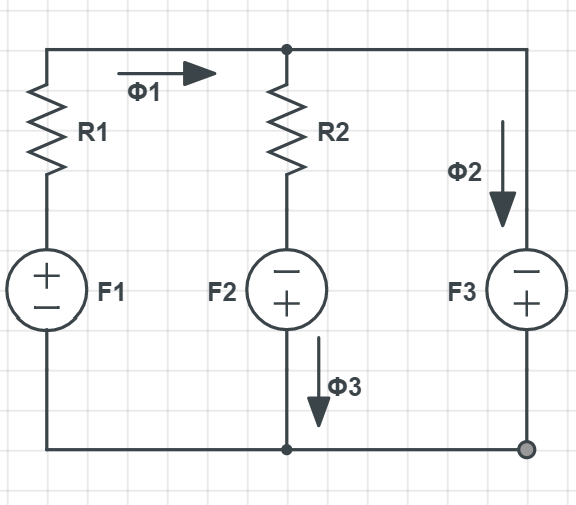
\includegraphics[scale=0.75]{33}

As equaçoes das malhas são as seguintes:
$$Circuito \ 1 : F_1 - \Re_1 \phi_1 - \Re_2 \phi_1 + \Re_2 \phi_2 + F_2 = 0$$
$$Circuito \ 2 :F_3 - \Re_2 \phi_2 + \Re_2 \phi_1 - F_2 = 0$$
$$\phi_1 - \phi_2 = \phi_3$$

Temos que $F_1 = F_2 = F_3 = NI$, pois todas as bobinas tem igual numero de espiras e corrente a percorrer. Assim os circuitos vão ser atualizados para:

$$Circuito \ 1 : 2F_1 - \phi_1(\Re_1 +\Re_2) + \Re_2 \phi_2 = 0$$
$$Circuito \ 2 : \Re_2 (\phi_1 - \phi_2) = 0 => \Re_2 \phi_3=0$$

Como sabemos que a relutancia $\Re_2$ e diferente de zero, temos que $\phi_3 = 0$ e por conseguinte $\phi_1 = \phi_2$.

Assim, voltando ao circuito 1 :

$$2F_1 - \phi_1 \Re_1 = 0$$
Substituindo F por NI e colocando o valor de relutancia magnetica encontrado na pergunta anterior, temos que:
$$\phi_1 = \phi_2 = \frac{2.315\times 10^{-7}}{l} \ [Wb]$$

\subsubsection{Calcule a energia magnética armazenada.}
A energia magnética armazenada pela passagem de corrente num indutor é igual à energia necessaria para produzir essa mesma corrente nesse mesmo indutor.
$$W_m = L \int idi = \frac{1}{2} L I^{2} = \frac{1}{2}[\psi]^{T}[I] $$
$$W_m = \frac{1}{2}[\psi_1 \ \psi_2 \ \psi_3][I_1 \ I_2 \ I_3]^{T} = \frac{1}{2}[\phi_1 N_1 \ \phi_2 N_2 \ \phi_3 N_3][I_1 \ I_2 \ I_3]^{T} $$ 

Como $N_1 = N_2 = N_3$ e $I_1 = I_2 = I_3$ temos que:
$$W_m = [\phi_1  \ \phi_2  \ \phi_3 ]\frac{NI}{2} = 375 [\phi_1  \ \phi_2  \ \phi_3 ] = 375 [\phi_1  \ \phi_2] = 375\times 2\times \phi_1 $$
Pegando no calculado na alinea anterior, temos que a Energia magnetica armazenada vai ser $\frac{1.7\times 10^{-4}}{l} [J]$

\subsubsection{Calcule a Indutância da fase e verifique o resultado da alinea anterior.}
Como vimos na alínea anterior: 
$$W_m = \frac{1}{2}LI^{2}$$
Assim:
$$L = \frac{2W_m}{I^{2}} = \frac{3.78 \times 10^{-4}}{l} {H}$$
\subsection{A seguinte figura contém um desenho de um motor IPM (significado: Interior Permanent Magnets) com as respectivas dimensoes assinaladas.}

\subsubsection{Desenhe o cirucito magnético equivalente e identifique as relutâncias com nomes apropriados, tal como os respectivos fluxos.}
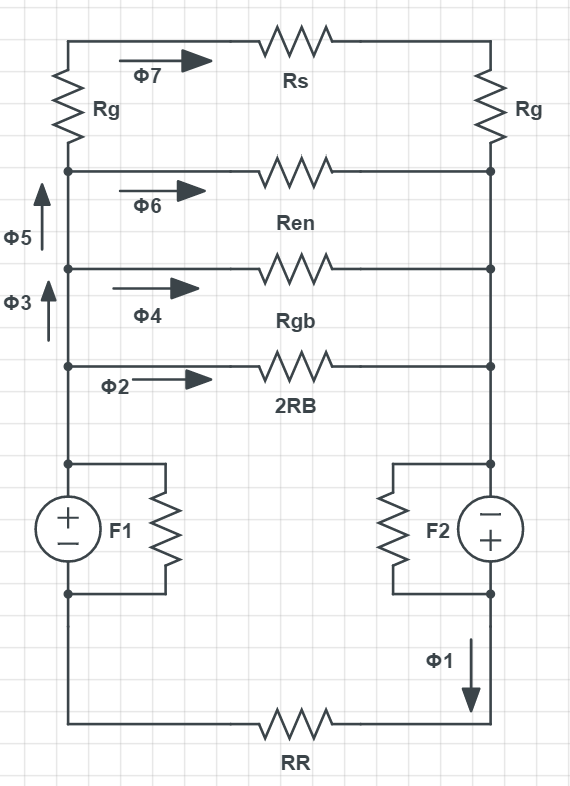
\includegraphics[scale=0.75]{66}

\begin{center}
    \begin{tabular}{ | l | l | l | p{5cm} |}
    \hline
    Simbolo & Termo \\ \hline
    RR & Relutancia do Rotor  \\ \hline
    RB & Relutancia da Barreira \\ \hline
    Rgb & Relutancia entre Barreira e gap (entreferro)  \\
    \hline
   Ren & Relutancia do entreferro  \\
    \hline
    Rg & Relutancia do Air Gap (direçao vertical)\\
    \hline
     Rs & Relutancia do estator\\
    \hline
       $\phi_1$ & Fluxo no Rotor\\
    \hline
     $\phi_2$ & Fluxo na barreira\\
    \hline
     $\phi_4$ & Fluxo entre o air gap e a barreira\\
    \hline
     $\phi_6$ & Fluxo no entreferro\\
    \hline
     $\phi_7$ & Fluxo no Estator, passando pelo air gap verticalmente\\
    \hline
    \end{tabular}
\end{center}

\subsubsection{Calcule o valor do campo mágnético médio na região do entreferro.}
Para calcular o campo magnético na região do entreferro (air-gap entre o estator e o rotor), temos que calcular o fluxo que passar por área nessa zona.

Tomando como referência o circuito apresentado na figura anterior, temos que o fluxo a passar nessa zona é o fluxo 6.

Para descobrirmos o fluxo que passa no entreferro, podemos pela lei das malhas considerar a malha que passa em RR, passa por F1, vai a Ren e volta para F2.

A equaçao correspondente a essa malha é a seguinte (F1 = F2):
$$-\phi_6 Ren + 2F - \phi_1 RR = 0$$

Para descobrirmos o $\phi_1$ podemos considerar uma relutancia equivalente R em serie com a relutancia do rotor RR:

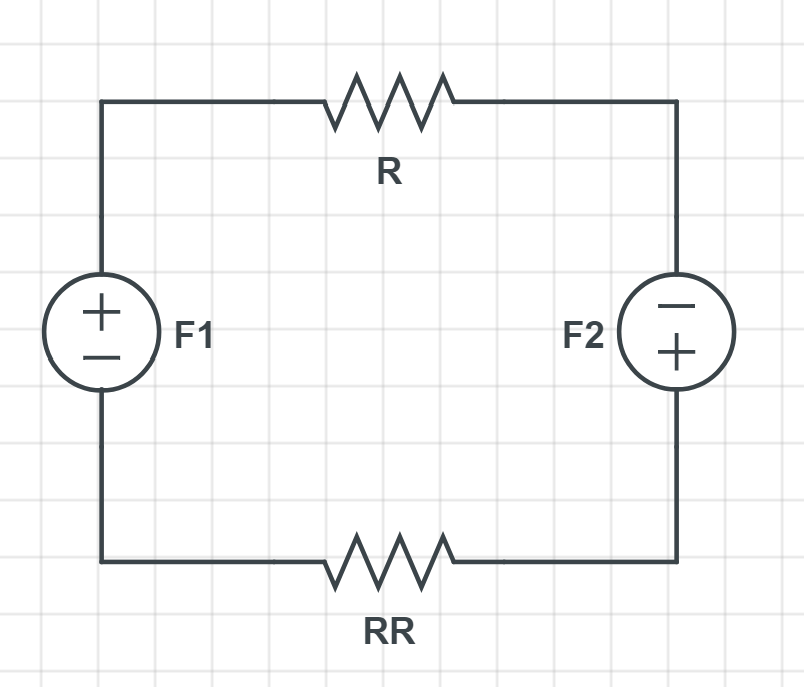
\includegraphics[scale=0.5]{44}

Primeiro temos de calcular cada resistência em específico.
$$RB = \frac{2d}{(AB)\times \mu_0}$$
$$RR = \frac{2d}{(AR)\times (\mu R)}$$
$$Rgb = \frac{2d}{(Agb)\times (\mu R)}$$
$$Ren = \frac{(len)}{(Aen)\times (\mu_0)}$$
$$Rg = \frac{(g)}{(Ag)\times (\mu_0)}$$
$$Rs = \frac{(ls)}{(As)\times (\mu S)}$$

Depois de ter calculado todas as relutancias, pode-se fazer o cálculo da resistência equivalente:
$$R = \frac{1}{\frac{1}{2Rg + Rs} + \frac{1}{Ren} + \frac{1}{Rg}+\frac{1}{2RB}}$$

Assim, o $$\phi_1$$ pode ser calculado:
$$\phi_1 = \frac{2F}{R+RR}$$

Voltando ao circuito considerado inicialmente temos que:
$$\phi_6 = \frac{2F - \phi_1RR}{Ren}$$

Pela definição de fluxo temos que $\phi = \int BdS$. Aplicando à nossa situacao:
$$B\times Aen = \phi_6 => B = \frac{\phi_6}{Aen}$$



\end{document}
